\chapter{Restitution interactive et visualisation}

\section{Introduction}

Ce chapitre présente la phase finale de l’analyse : la restitution interactive des résultats à travers un tableau de bord conçu avec Power BI. 
L’objectif est de permettre une exploration dynamique et intuitive des données du baccalauréat sénégalais de 2006 à 2024, 
à destination notamment de l’Office du Baccalauréat et de toute personne souhaitant approfondir une étude sur le sujet.

\section{objectifs du dashboard}

Le tableau de bord a pour but :

\begin{itemize}
    \item de synthétiser les indicateurs clés liés au taux de réussite au baccalauréat par année, série et session ;
    \item d’observer l’évolution de ces indicateurs dans le temps ;
    \item de permettre un filtrage dynamique selon les besoins d’analyse ;
    \item et de soutenir la prise de décision à travers des visualisations claires et interactives.
\end{itemize}

\section{Présentation des indicateurs suivis}

Les indicateurs principaux intégrés dans le dashboard sont :
\begin{itemize}
    \item Le taux de réussite global par année ;
    \item Le taux de réussite par série ;
    \item Le nombre total d’admis et d’inscrits ;
    \item La répartition par session (1er ou 2e tour) ;
    \item La répartition par mention obtenue.
\end{itemize}

\newpage
\section{Construction du dashboard Power BI}

\subsection{Première version : Résultats de 2024 uniquement}

Dans un premier temps, n’ayant pas encore accès à l’ensemble des données historiques, 
j’ai construit une première version du tableau de bord en me basant uniquement sur les résultats de l’année 2024. 
Cette version m’a permis de tester la structure du dashboard et de définir les visualisations pertinentes à suivre. 
Elle comportait déjà tous les indicateurs énumérés précédemment.
\vspace{1cm}
\begin{figure}[htbp]
    \centering
    \caption{Tableau de bord Power BI - Résultats du baccalauréat 2024}
    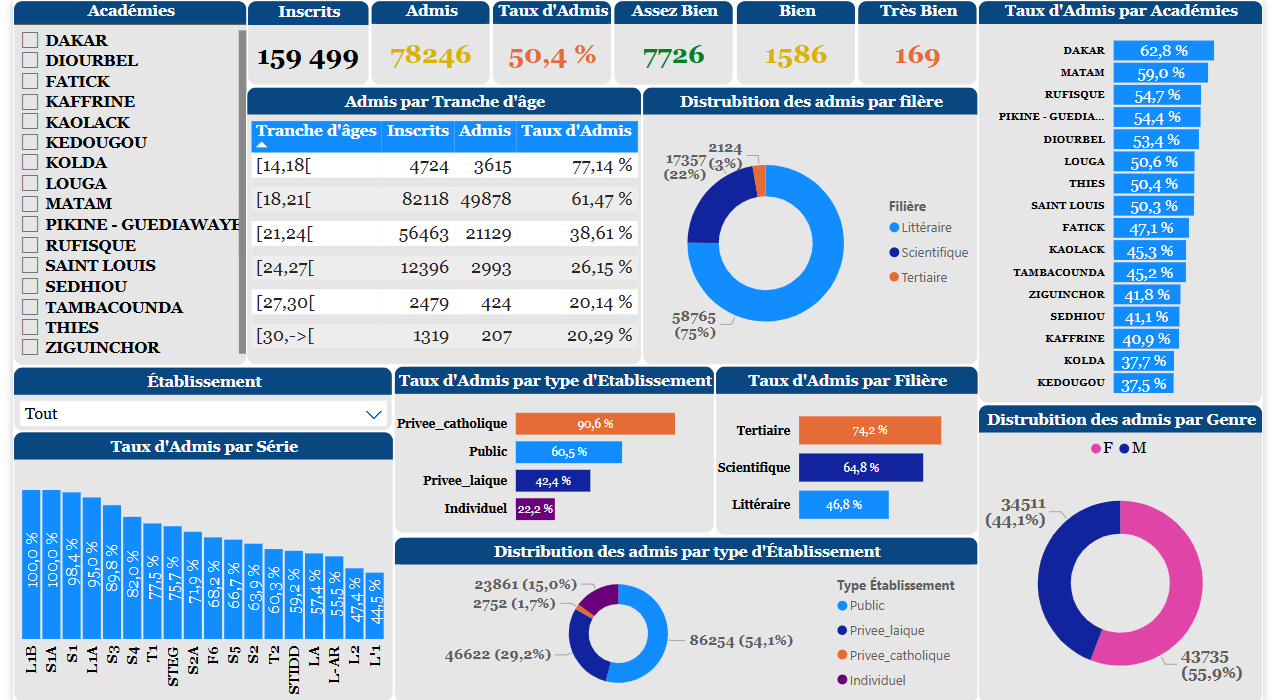
\includegraphics[width=15cm]{figure/bac_2024.png}
\end{figure}

\newpage
\subsection{ Deuxième version : Résultats de 2006 à 2024}

Une fois l’accès aux données complètes obtenu, j’ai pu enrichir le dashboard avec les résultats du bac de 2006 à 2024. 
Cette version permet d’analyser l’évolution temporelle des indicateurs clés et de mieux comprendre l’impact des différentes réformes au fil des années.
\vspace{1cm}
\begin{figure}[htbp]
    \centering
    \caption{Tableau de bord Power BI - Résultats du baccalauréat 2006 à 2024}
    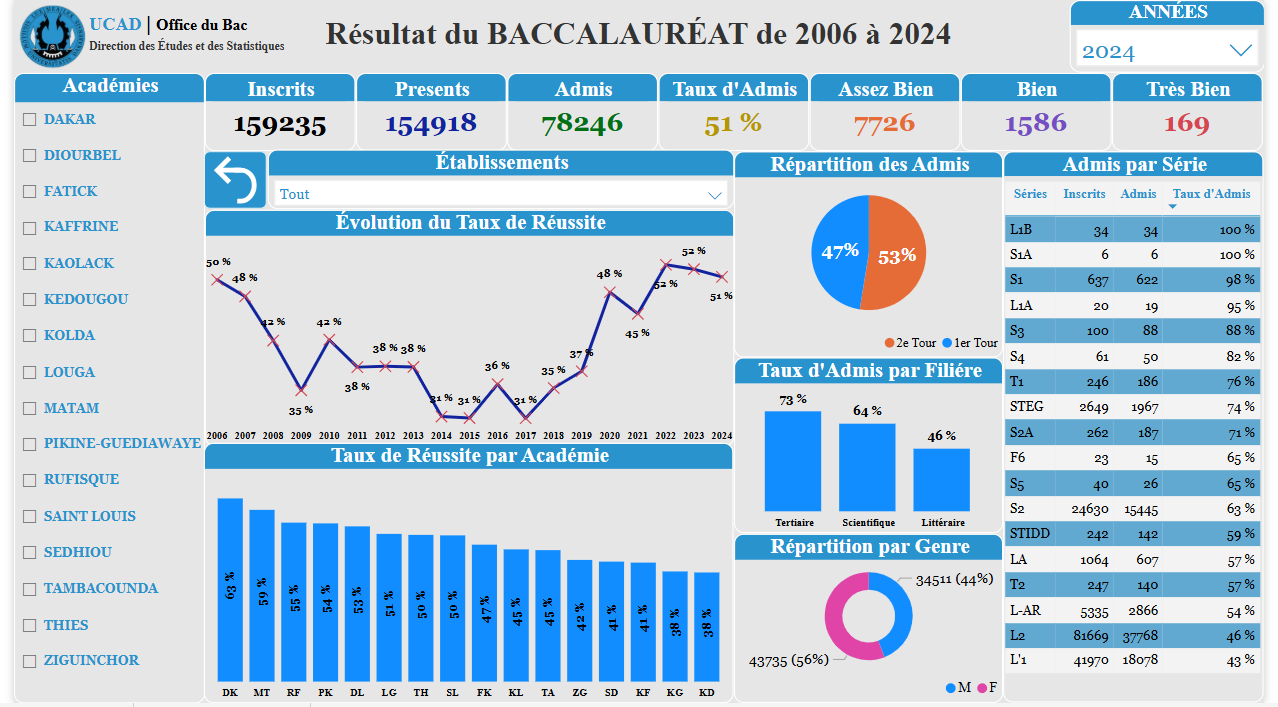
\includegraphics[width=15cm]{figure/bac_2006_2024.png}
\end{figure}

\newpage
\subsection{Utilisation de Power Query et création de mesures}

Power Query a été utilisé pour nettoyer et transformer les données importées dans Power BI. 
J’y ai notamment créé des colonnes conditionnelles pour catégoriser les mentions ou les sessions, 
et j’ai défini plusieurs mesures DAX (Data Analysis Expressions) telles que le taux de réussite, 
le nombre total d’inscrits ou encore les ratios d’admis par série.

\section{Conclusion}

La restitution interactive via Power BI offre une approche moderne et intuitive de l’analyse des données du baccalauréat. 
Elle facilite l’interprétation des tendances et appuie la prise de décision à partir d’une lecture visuelle et dynamique des résultats. 
Ce tableau de bord constitue un apport concret à l’Office du Baccalauréat, pouvant soutenir les futures études sur l’évolution du système éducatif au Sénégal.